%%%%%%%%%%%%%%%%%%%%%
% 5章
%%%%%%%%%%%%%%%%%%%%%
\chapter{計算機実験} \label{chapter:5}

\section{概要}
本章では,提案手法であるヒューリスティクス解を用いたZDD構築の
計算機実験を行い,既存手法の人口制約のないZDD構築手法,
人口制約ありで許容格差定数を用いたZDD構築手法との比較をし,
提案手法の評価及び考察を行う.

\section{実験環境}
実験環境は,次の通りである.

\begin{itemize}
  \item OS:Ubuntu 20.04.5 LTS
  \item CPU:Intel Xeon E5-2687W v4(3.0GHz)
  \item メモリ:512GB
\end{itemize}

プログラムはC++17によって実装し,gccを用いて -O3, -march=native
オプションを付与してコンパイルを行った.また,ライブラリとして,
SAPPOROBDD,TdZdd を利用した.

\section{入力データ}
入力データとして,国土交通省が公開している「国土数値情報 行政区域データ」と
令和2年国勢調査結果の「人口等基本集計」を利用し,
市区町村を頂点,隣接関係を辺,人口を頂点重みとした
グラフを作成した.
本論文ではいくつかの都道府県のインスタンスを抜粋して掲載する.
入力データについて,各インスタンスのパラメータを表\ref{input_data}にまとめた.

\begin{table}[htbp]
  \caption{入力データ}
  \label{input_data}
  \centering
  \begin{tabular}{l|rrr}
    \hline
    Name & $|V|$ & $|E|$ & $d$ \\
    \hline \hline
    $G_1$(Aomori) & 40 & 84 & 3 \\
    $G_2$(Miyagi) & 39 & 86 & 5 \\
    $G_3$(Yamagata) & 35 & 85 & 3 \\
    $G_4$(Fukushima) & 59 & 144 & 4 \\
    $G_5$(Ibaraki) & 44 & 94 & 7 \\
    $G_6$(Nagano) & 77 & 187 & 5 \\
    $G_7$(Aichi) & 69 & 173 & 16 \\
    $G_8$(Osaka) & 72 & 168 & 19 \\
    \hline
  \end{tabular}
\end{table}

表\ref{input_data}の$|V|$は頂点数,$|E|$は辺数,$d$は分割数を
表している.
また,頂点の各重みについて分布図を図\ref{w_dist}にまとめた.

\begin{figure}[bp]
  \begin{tabular}{cc}
    \begin{minipage}[t]{0.45\hsize}
      \centering
      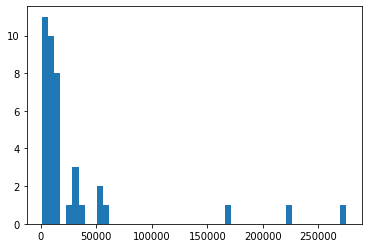
\includegraphics[keepaspectratio, scale=0.5]{img/g1.png}
      \subcaption{$G_1$}
      \label{g1}
    \end{minipage} &
    \begin{minipage}[t]{0.45\hsize}
      \centering
      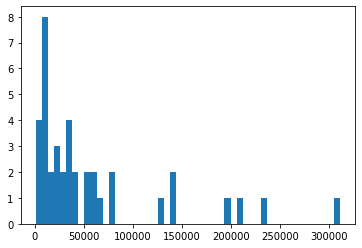
\includegraphics[keepaspectratio, scale=0.5]{img/g2.png}
      \subcaption{$G_2$}
      \label{g2}
    \end{minipage} \\

    \begin{minipage}[t]{0.45\hsize}
      \centering
      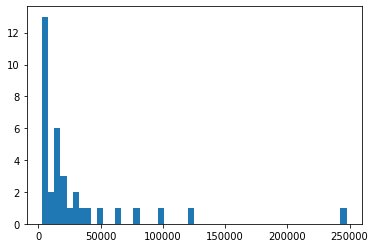
\includegraphics[keepaspectratio, scale=0.5]{img/g3.png}
      \subcaption{$G_3$}
      \label{g3}
    \end{minipage} &
    \begin{minipage}[t]{0.45\hsize}
      \centering
      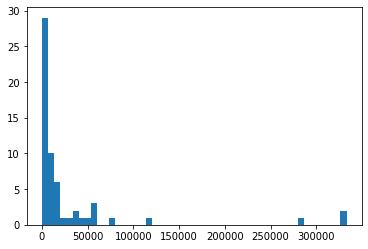
\includegraphics[keepaspectratio, scale=0.5]{img/g4.png}
      \subcaption{$G_4$}
      \label{g4}
    \end{minipage} \\
    \begin{minipage}[t]{0.45\hsize}
      \centering
      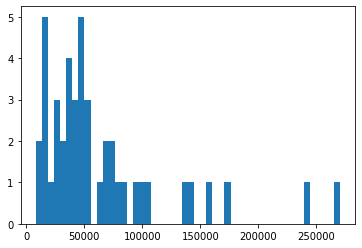
\includegraphics[keepaspectratio, scale=0.5]{img/g5.png}
      \subcaption{$G_5$}
      \label{g5}
    \end{minipage} &
    \begin{minipage}[t]{0.45\hsize}
      \centering
      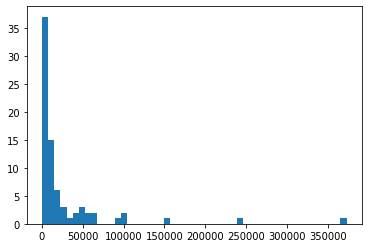
\includegraphics[keepaspectratio, scale=0.5]{img/g6.png}
      \subcaption{$G_6$}
      \label{g6}
    \end{minipage} \\

    \begin{minipage}[t]{0.45\hsize}
      \centering
      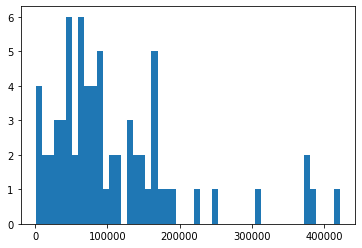
\includegraphics[keepaspectratio, scale=0.5]{img/g7.png}
      \subcaption{$G_7$}
      \label{g7}
    \end{minipage} &
    \begin{minipage}[t]{0.45\hsize}
      \centering
      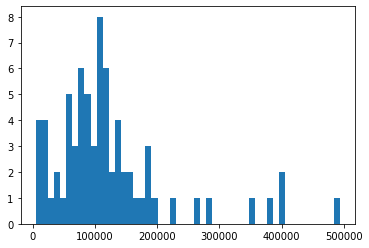
\includegraphics[keepaspectratio, scale=0.5]{img/g8.png}
      \subcaption{$G_8$}
      \label{g8}
    \end{minipage}
  \end{tabular}
  \caption{頂点の重み分布}
  \label{w_dist}
\end{figure}


\section{実験結果}

\subsection{人口制約なし}

3.3.1項にて述べた人口制約のない区割列挙の結果は,
表\ref{out_normal}の通りである.

\begin{table}[htbp]
  \caption{人口制約なし区割列挙}
  \label{out_normal}
  \centering
  \begin{tabular}{l||r|r|r|r}
    \hline
    Name & node & solve & time(sec) & memory(MB) \\
    \hline \hline
    $G_1$(Aomori) & 5196 & 10452641 & 0.02 & 6 \\
    $G_2$(Miyagi) & 2891 & 1.98E+10 & 0.01 & 4 \\
    $G_3$(Yamagata) & 2672 & 490516246 & 0.01 & 4 \\
    $G_4$(Fukushima) & 233446 & 1.51E+14 & 1108.69 & 16859 \\
    $G_5$(Ibaraki) & 10757 & 3.24E+13 & 0.02 & 6 \\
    $G_6$(Nagano) & 48612 & 3.82E+17 & 1.48 & 472 \\
    $G_7$(Aichi) & 1145106 & 3.02E+29 & 2.41 & 395 \\
    $G_8$(Osaka) & 955147 & 1.73E+30 & 0.5 & 92 \\
    \hline
  \end{tabular}
\end{table}


\subsection{人口制約あり:許容格差定数を用いる場合}

\begin{table}[htbp]
  \caption{$r=1.4$とした区割列挙}
  \label{out_r}
  \centering
  \begin{tabular}{l||r|r||r|r|r|r}
    \hline
    Name & $L$ & $U$ & node & solve & time(sec) & memory(MB) \\
    \hline \hline
    $G_1$(Aomori) & 325785 & 509759 & 23749 & 668154 & 2.25 & 405 \\
    $G_2$(Miyagi) & 348787 & 596814 & 6581 & 40106 & 3.38 & 652 \\
    $G_3$(Yamagata) & 281059 & 439776 & 319171 & 7493473 & 33.81 & 6702 \\
    $G_4$(Fukushima) & 585129 & 353649 & N/A & N/A & N/A & N/A \\
    $G_5$(Ibaraki) & 305000 & 542408 & 1077156 & 36745326 & 212.75 & 30690 \\
    $G_6$(Nagano) & 310304 & 530966 & N/A & N/A & N/A & N/A \\
    $G_7$(Aichi) & 342837 & 643865 & N/A & N/A & N/A & N/A \\
    $G_8$(Osaka) & 337316 & 637772 & N/A & N/A & N/A & N/A \\
    \hline
  \end{tabular}
\end{table}


\subsection{人口制約あり:ヒューリスティクスの結果を用いる場合}

\begin{table}[htbp]
  \caption{ヒューリスティクスを用いた区割列挙}
  \label{out_h}
  \centering
  \begin{tabular}{l||r|r||r|r|r|r}
    \hline
    Name & $L$ & $U$ & node & solve & time(sec) & memory(MB) \\
    \hline \hline
    $G_1$(Aomori) & 226194 & 555698 & 34609 & 2001248 & 2.77 & 460 \\
    $G_2$(Miyagi) & 451162 & 467561 & 55 & 2 & 0.01 & 4 \\
    $G_3$(Yamagata) & 355396 & 356505 & 4416 & 541 & 0.08 & 19 \\
    $G_4$(Fukushima) & 459096 & 460480 & N/A & N/A & N/A & N/A \\
    $G_5$(Ibaraki) & 391937 & 419212 & 1340 & 390 & 0.02 & 6 \\
    $G_6$(Nagano) & 408772 & 410752 & 10320 & 17657 & 2.3 & 471 \\
    $G_7$(Aichi) & 359399 & 553700 & 1847085 & 1.29E+14 & 89.02 & 12607 \\
    $G_8$(Osaka) & 424530 & 569011 & N/A & N/A & N/A & N/A \\
    \hline
  \end{tabular}
\end{table}


\section{考察}